\chapter{From Equilibrium State to Device Prediction}
\label{ch:equilibrium-to-device-prediction}

A device calculation must begin from a defined material state.  Carrier
concentrations, chemical potentials, band gaps, masses, and dopant charge states
come from equilibrium statistics.  Mobility, lifetime, surface recombination,
contact resistance, and impact ionization require additional constitutive data.
This chapter makes that division explicit and connects the equilibrium model of
Chapters~4--7 to the transport and p--n-junction models of
Chapters~12--20.  It also supplies the generalized Einstein relation,
incomplete-ionization corrections to depletion charge, and a reproducible
calibration, validation, and uncertainty workflow
\cite[Chaps.~2--3]{szeLee2012} \cite[Chaps.~1--2]{szeNg2007}.

\section{The equilibrium-to-device data contract}

\begin{definition}{Transferred equilibrium state}{transferred-equilibrium-state}
A transferred equilibrium state is a machine-readable record of one homogeneous
material at a declared temperature and nominal donor and acceptor concentration.
It contains the electron density $n$, hole density $p$, chemical potential
$\mu$, intrinsic density $n_i$, band gap $E_g$, ionized donor density $N_D^+$,
ionized acceptor density $N_A^-$, and charge-neutrality residual, together with
the energy reference and parameter provenance.
\end{definition}

The transfer must preserve definitions, not only numerical values.  A useful
minimum row is
\begin{equation}
 \mathcal S=
 \{T,N_D,N_A,N_D^+,N_A^-,n,p,\mu,n_i,E_g,r_{\mathrm{neutral}}\}.
 \label{eq:equilibrium-state-record}
\end{equation}
The record must identify the exact material phase or polytype and the source
revision of the equilibrium calculation.  Effective-mass tensors, valley
counts, band edges, dopant levels, and degeneracy conventions belong in an
accompanying parameter record.

The first device calculation is therefore an audit:
\begin{align}
 p+N_D^+-n-N_A^-&=r_{\mathrm{neutral}}\simeq0,
 \label{eq:transferred-neutrality-check}\\
 np&=n_i^2
 \quad\text{when nondegenerate mass action applies}.
 \label{eq:transferred-mass-action-check}
\end{align}
A result outside the validated temperature or concentration range of the
parent equilibrium model is not repaired by a more elaborate device solver.

\section{Inherited state and newly introduced physics}

The equilibrium record supplies carrier populations and dopant charge states.
It does not supply momentum or energy relaxation.  The low-field conductivity
requires new mobilities,
\begin{equation}
 \sigma=q(n\mu_n+p\mu_p),
 \label{eq:integrated-conductivity}
\end{equation}
and mobility requires a scattering model or measured data.  Effective mass
alone gives only
\begin{equation}
 \mu=\frac{q\tau_m}{m_c^*},
 \label{eq:integrated-mobility}
\end{equation}
so an absolute prediction still requires momentum-relaxation time $\tau_m$.
Likewise, diffusion length requires a lifetime that is not fixed by equilibrium
statistics:
\begin{equation}
 L_n=\sqrt{D_n\tau_n},
 \qquad
 L_p=\sqrt{D_p\tau_p}.
 \label{eq:integrated-diffusion-length}
\end{equation}

A transparent prediction table separates three input classes:
\begin{center}
\small
\begin{tabularx}{\textwidth}{@{}>{\raggedright\arraybackslash}p{0.21\textwidth}>{\raggedright\arraybackslash}p{0.34\textwidth}>{\raggedright\arraybackslash}X@{}}
\toprule
Class & Examples & Required evidence \\
\midrule
Inherited equilibrium state & $E_g$, $n_i$, $n$, $p$, $\mu$, $N_D^+$, $N_A^-$, masses and valleys & Parent calculation, neutrality residual, provenance, and file hash \\
New constitutive physics & $\mu_n$, $\mu_p$, $r_H$, $\tau_n$, $\tau_p$, $S$, $\alpha_n$, $\alpha_p$, $R_s$ & Independent measurement, literature model, or explicitly calibrated relation \\
Declared device model & Area, orientation, neutral lengths, contacts, bias, boundary conditions & Geometric specification and physical justification \\
\bottomrule
\end{tabularx}
\end{center}

\section{Built-in potential from the two bulk chemical potentials}

Consider isolated n-type and p-type regions of the same semiconductor at the
same temperature.  Their band edges use one common energy reference.  Before
contact, let their chemical potentials be $\mu_n^{\mathrm{bulk}}$ and
$\mu_p^{\mathrm{bulk}}$.  After contact, electrostatic band bending makes the
electrochemical potential spatially constant.  The required contact-potential
difference is
\begin{equation}
 \boxed{
 qV_{\mathrm{bi}}
 =\mu_n^{\mathrm{bulk}}-\mu_p^{\mathrm{bulk}}.
 }
 \label{eq:built-in-from-chemical-potentials}
\end{equation}
The energies on the right must be expressed in joules when $q$ is retained.
When they are expressed in electron-volts, their numerical difference equals
$V_{\mathrm{bi}}$ in volts.

A common energy-reference shift $E\mapsto E+E_0$ changes both chemical
potentials by $E_0$ and leaves their difference unchanged:
\begin{equation}
 (\mu_n+E_0)-(\mu_p+E_0)=\mu_n-\mu_p.
 \label{eq:built-in-energy-shift-invariance}
\end{equation}
This invariance is an essential transfer test.

In the nondegenerate limit,
\begin{equation}
 \mu_n-\mu_i=k_BT\ln\left(\frac{n_{n0}}{n_i}\right),
 \qquad
 \mu_i-\mu_p=k_BT\ln\left(\frac{p_{p0}}{n_i}\right),
 \label{eq:bulk-chemical-potentials-carriers}
\end{equation}
where $n_{n0}$ is the equilibrium electron density in the n-type bulk and
$p_{p0}$ is the equilibrium hole density in the p-type bulk.  Adding the two
relations gives
\begin{equation}
 \boxed{
 V_{\mathrm{bi}}
 =V_T\ln\left(\frac{n_{n0}p_{p0}}{n_i^2}\right).
 }
 \label{eq:built-in-from-transferred-carriers}
\end{equation}
Only after assuming complete ionization and strong majority-carrier behavior
may one replace $n_{n0}$ by $N_D$ and $p_{p0}$ by $N_A$ to recover
\cref{eq:pn-built-in-potential}.

\section{Incomplete ionization inside the depletion model}

The exact junction charge is
\begin{equation}
 \rho(x)=q\left[p(x)-n(x)+N_D^+(x)-N_A^-(x)\right].
 \label{eq:ionization-aware-junction-charge}
\end{equation}
There are three distinct approximation levels.

\begin{enumerate}
 \item \textbf{Complete ionization:}
 $N_D^+=N_D$ and $N_A^-=N_A$.  This is the standard textbook depletion model.
 \item \textbf{Frozen transferred ionization:}
 use the bulk values $N_D^+(T,\mu_n^{\mathrm{bulk}})$ and
 $N_A^-(T,\mu_p^{\mathrm{bulk}})$ throughout each depleted side.  This imports
 the equilibrium charge-state result but neglects its response to band bending.
 \item \textbf{Local-equilibrium ionization:}
 evaluate $N_D^+[\mu-E_D(x),T]$ and $N_A^-[E_A(x)-\mu,T]$ locally inside the
 nonlinear Poisson equation.  This is required when depletion substantially
 changes dopant occupation.
\end{enumerate}

Under the frozen-ionization depletion approximation,
\begin{equation}
 N_A^-x_p=N_D^+x_n,
 \label{eq:ionized-depletion-neutrality}
\end{equation}
and
\begin{equation}
 \boxed{
 W=\sqrt{\frac{2\varepsilon_s}{q}(V_{\mathrm{bi}}-V)
 \left(\frac{1}{N_A^-}+\frac{1}{N_D^+}\right)}.
 }
 \label{eq:ionized-depletion-width}
\end{equation}
The capacitance remains $C_j=\varepsilon_s/W$.  In a one-sided junction whose
lightly doped side has ionized fraction $f$, one obtains
\begin{equation}
 \frac{W}{W_{\mathrm{full}}}=f^{-1/2},
 \qquad
 \frac{C_j}{C_{j,\mathrm{full}}}=f^{1/2}.
 \label{eq:ionization-depletion-scaling}
\end{equation}
Nominal dopant density and electrically active depletion charge are therefore
not interchangeable.

\section{Generalized Einstein relation}

The classical relation $D=\mu V_T$ assumes a nondegenerate gas.  More generally,
a carrier flux responds to the gradient of electrochemical potential.  For an
isothermal electron population with chemical potential $\mu_c(n,T)$,
thermodynamic consistency gives
\begin{equation}
 \boxed{
 \frac{D_n}{\mu_n}
 =\frac{n}{q}\left(\frac{\partial\mu_c}{\partial n}\right)_T.
 }
 \label{eq:generalized-einstein-thermodynamic}
\end{equation}
The derivative uses energy units.  In the Boltzmann limit,
$\mu_c=\mathrm{constant}+k_BT\ln n$, so the right-hand side becomes
$k_BT/q=V_T$.

For a three-dimensional parabolic conduction band,
\begin{equation}
 n=N_C\mathcal F_{1/2}(\eta_n),
 \qquad
 \eta_n=\frac{\mu-\Ec}{k_BT},
 \label{eq:fermi-density-reduced-potential}
\end{equation}
where $\mathcal F_j$ is the normalized complete Fermi--Dirac integral.  Since
$\partial\mathcal F_{1/2}/\partial\eta=\mathcal F_{-1/2}$ under this convention,
\begin{equation}
 \boxed{
 \frac{D_n}{\mu_n}
 =V_T\frac{\mathcal F_{1/2}(\eta_n)}
 {\mathcal F_{-1/2}(\eta_n)}.
 }
 \label{eq:generalized-einstein-fermi}
\end{equation}
An analogous expression applies to holes with
$\eta_p=(\Ev-\mu)/(k_BT)$.  The ratio approaches one far from a band edge and
rises under degeneracy.  Hall mobility must not be substituted for drift
mobility unless the Hall factor has first been removed.

\section{Calibration, validation, and prediction}

\begin{definition}{Calibration and validation}{calibration-validation}
\emph{Calibration data} determine an uncertain parameter or model coefficient.
\emph{Validation data} test the resulting model without being used to choose
that parameter.  A \emph{prediction} applies the calibrated and validated model
to a declared state or geometry not already fixed by those data.
\end{definition}

A mobility curve fitted to one sample is calibration evidence.  Reproducing the
same curve is not an independent validation.  A defensible workflow is:

\begin{enumerate}
 \item freeze and audit the equilibrium-state transfer;
 \item select mobility and lifetime sources with valid ranges;
 \item calibrate only the parameters that the chosen data can identify;
 \item test analytic limits, conservation, residuals, and grid convergence;
 \item compare with independent transport or device data;
 \item predict one declared operating point; and
 \item report the range in which every input model remains valid.
\end{enumerate}

Parameter identifiability matters.  The ideal saturation current contains
combinations such as
\begin{equation}
 J_s=q\left[
 n_{p0}\sqrt{\frac{D_n}{\tau_n}}
 +p_{n0}\sqrt{\frac{D_p}{\tau_p}}
 \right]
 \label{eq:integrated-long-base-saturation-current}
\end{equation}
for a long-base junction.  One measured $J_s$ cannot independently determine
both diffusivities and both lifetimes.

\section{Uncertainty propagation and sensitivity}

Let an output $y=f(\bm\theta)$ depend on parameters
$\bm\theta=(\theta_1,\ldots,\theta_m)$.  A local dimensionless sensitivity is
\begin{equation}
 S_i=\frac{\partial\ln y}{\partial\ln\theta_i}.
 \label{eq:local-log-sensitivity}
\end{equation}
For small independent uncertainties,
\begin{equation}
 \left(\frac{u_y}{y}\right)^2
 \simeq\sum_i S_i^2
 \left(\frac{u_{\theta_i}}{\theta_i}\right)^2.
 \label{eq:first-order-uncertainty}
\end{equation}
A covariance matrix must replace this sum when inputs share a source or fitted
model.

The ideal current is exponentially sensitive to band gap because
$n_i^2\propto\exp[-E_g/(k_BT)]$.  At
$T=\SI{300}{\kelvin}$, a
$\SI{10}{\milli\electronvolt}$ gap change alters the ideal $n_i^2$ scale by
approximately $39\%$.  By contrast, because
$\sqrt{D/\tau}$ enters \cref{eq:integrated-long-base-saturation-current}, a
$10\%$ mobility change produces approximately a $5\%$ current change when one
term dominates.  Sensitivity ranking therefore prevents equal attention being
given to unequal uncertainty sources.

When linear propagation is inadequate, draw correlated parameter samples,
rerun the complete deterministic model, and report the output distribution.
The sample ranges must represent evidence, not arbitrary percentages selected
after seeing the result.

\section{Integrated silicon and gallium-arsenide controls}

The Long Assessment 2 examples apply one transparent workflow to Si and GaAs.
At $\SI{300}{\kelvin}$, their illustrative nondegenerate controls give
\begin{center}
\small
\begin{tabular}{@{}lrrrr@{}}
\toprule
Material & $n_i$ ($\mathrm{cm^{-3}}$) & $V_{\mathrm{bi}}$ (V) & $W_0$ ($\mu$m) & $J_s$ ($\mathrm{A\,m^{-2}}$) \\
\midrule
Si & $6.12\times10^9$ & $0.799$ & $0.337$ & $7.14\times10^{-9}$ \\
GaAs & $2.04\times10^6$ & $1.213$ & $0.436$ & $8.79\times10^{-14}$ \\
\bottomrule
\end{tabular}
\end{center}
The comparison uses $N_A=10^{23}\,\mathrm{m^{-3}}$ and
$N_D=10^{22}\,\mathrm{m^{-3}}$.  The example lifetimes are
$\SI{10}{\micro\second}$ for Si and $\SI{1}{\nano\second}$ for GaAs.  Those
lifetimes are declared instructional inputs, not universal material constants.
They produce example minority-hole diffusion lengths of approximately
$\SI{105}{\micro\meter}$ and $\SI{0.97}{\micro\meter}$, respectively.

For an ideal finite-base current density of $10^4\,\mathrm{A\,m^{-2}}$, the
examples predict forward voltages near $\SI{0.723}{\volt}$ for Si and
$\SI{1.015}{\volt}$ for GaAs.  These values illustrate propagation through the
model chain.  They are not predictions for unspecified real diodes, whose
leakage, lifetime, surface condition, contacts, and geometry may differ.

\begin{figure}[htbp]
 \centering
 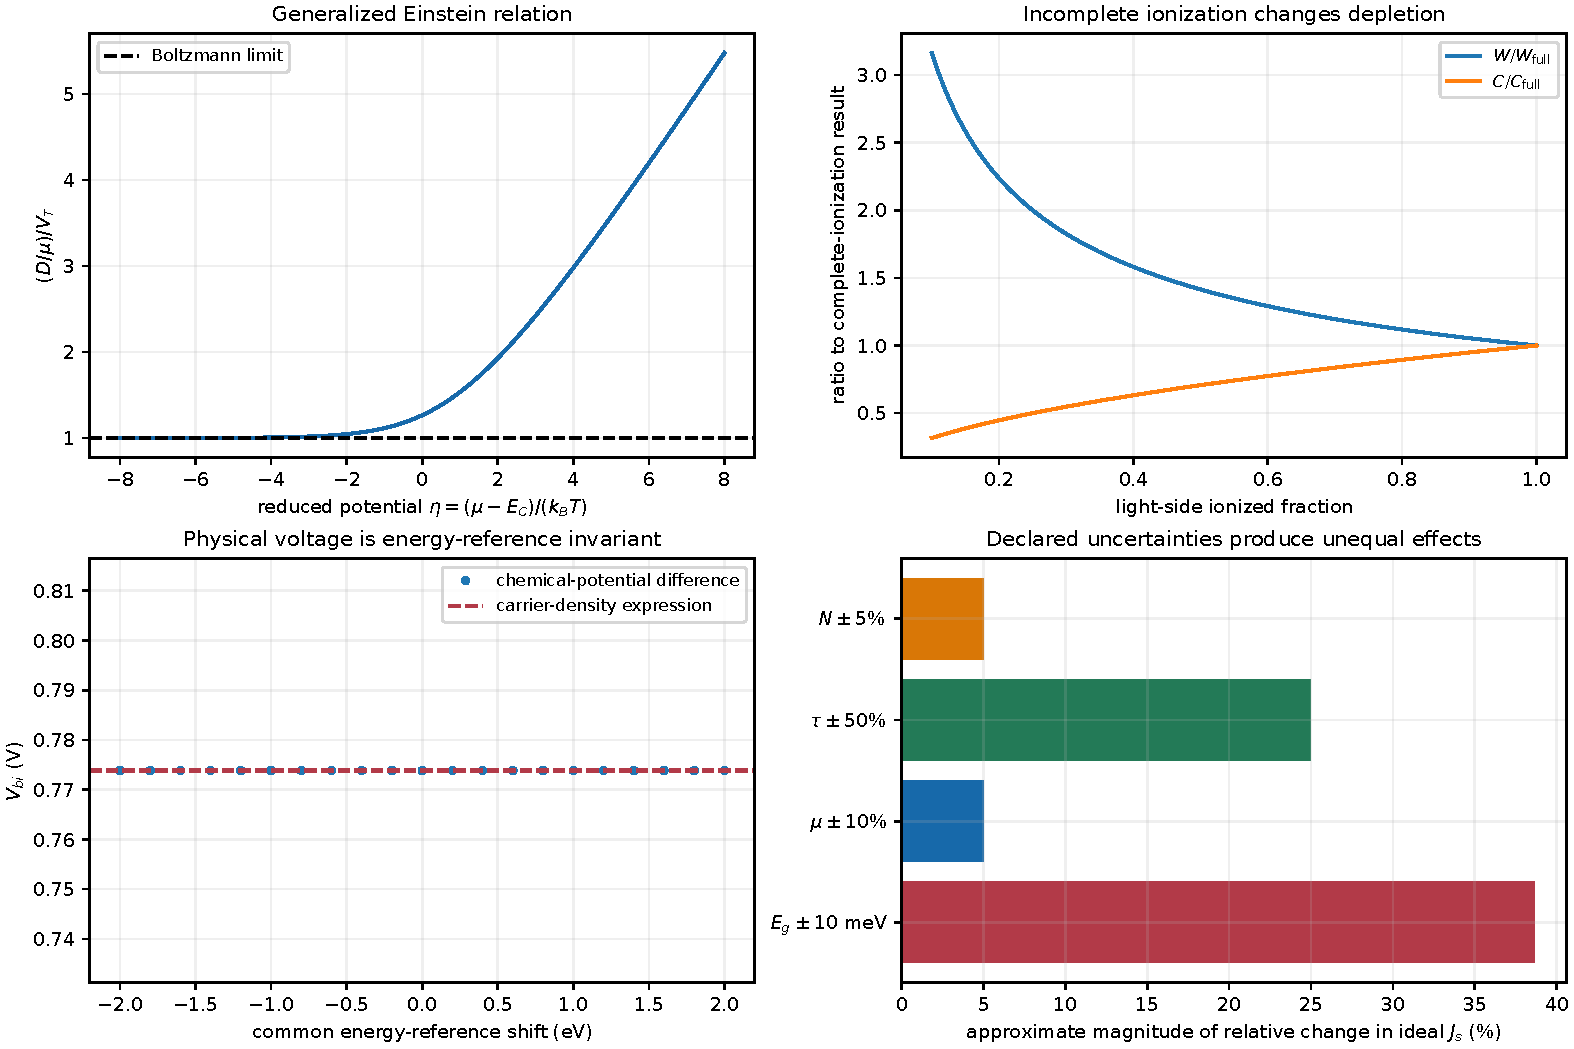
\includegraphics[width=\textwidth]{figures/device-prediction-integration.pdf}
 \caption{Generalized Einstein correction, incomplete-ionization effects on
 depletion width and capacitance, energy-reference invariance of built-in
 potential, and an illustrative uncertainty ranking for ideal saturation
 current.\figurenotebookmark}
 \label{fig:device-prediction-integration}
\end{figure}
\figurenotebooktext{figures/21_integrated-device-prediction/fig_21_01.ipynb}

\section{Integrated verification checklist}

A complete equilibrium-to-device prediction should verify:

\begin{enumerate}
 \item source-file hashes and transferred-state schema;
 \item charge neutrality and applicable mass action;
 \item invariance under a common energy-reference shift;
 \item mobility definitions, directions, and valid ranges;
 \item drift versus Hall mobility conventions;
 \item classical or generalized Einstein consistency;
 \item low-level-injection validity;
 \item continuity residual, positivity, convergence, and charge conservation;
 \item depletion charge neutrality using $N_D^+$ and $N_A^-$;
 \item agreement of chemical-potential and carrier-density built-in voltages;
 \item Poisson residual and electrostatic grid convergence;
 \item $C_jW=\varepsilon_s$ in the depletion limit;
 \item zero diode current at zero bias;
 \item analytic and numerical minority-current agreement;
 \item separation of calibration and validation data; and
 \item output sensitivity to inherited and newly introduced parameters.
\end{enumerate}

\section{Chapter summary}

Equilibrium carrier statistics define the material state from which transport
and junction prediction begins.  The built-in voltage is the difference of two
bulk chemical potentials expressed in one energy reference.  Incomplete
ionization changes fixed depletion charge and therefore changes width and
capacitance.  Degenerate carriers require a thermodynamic Einstein relation
rather than $D=\mu V_T$.  Mobility and lifetime remain new constitutive inputs,
not consequences of effective mass and carrier density alone.  Calibration,
independent validation, sensitivity, and uncertainty complete the chain from a
reproducible equilibrium state to a defensible device prediction.
